\section*{2.5 线性无关}
\addcontentsline{toc}{section}{2.5 线性无关}
\label{sec:2.5}

在下文中，我们将仔细考察可以对向量（向量空间中的元素）进行哪些操作。具体而言，我们可以将向量相加，也可以将它们乘以标量。封闭性保证了运算的结果仍然是同一向量空间中的另一个向量。我们有可能找到一组向量，使得通过对它们进行加法和缩放运算，能够表示该向量空间中的任意向量。这组向量构成了一组 \emph{基（basis）} ，我们将在第 2.6.1 节中对此进行详细讨论。在此之前，我们需要首先引入 \emph{线性组合（linear combinations）} 与 \emph{线性无关（linear independence）} 的概念。

\textbf{定义 2.11}（线性组合）。考虑一个向量空间 $ V $ 以及有限个向量 $ \boldsymbol{x}_1, \ldots, \boldsymbol{x}_k \in V $。那么，形式如下的任意向量 $ \boldsymbol{v} \in V $：

\begin{equation}
\boldsymbol{v} = \lambda_1 \boldsymbol{x}_1 + \cdots + \lambda_k \boldsymbol{x}_k = \sum_{i=1}^k \lambda_i \boldsymbol{x}_i \in V
\tag{2.65}\label{eq:2-65}
\end{equation}

其中 $ \lambda_1, \ldots, \lambda_k \in \mathbb{R} $，称为向量 $ \boldsymbol{x}_1, \ldots, \boldsymbol{x}_k $ 的 \emph{线性组合（linear combination）} 。

零向量 $ \boldsymbol{0} $ 总是可以表示为 $ k $ 个向量 $ \boldsymbol{x}_1, \ldots, \boldsymbol{x}_k $ 的线性组合，因为 $ \boldsymbol{0} = \sum_{i=1}^k 0 \boldsymbol{x}_i $ 始终成立。在下文中，我们感兴趣的是使用一组向量表示 $ \boldsymbol{0} $ 的 \emph{非平凡线性组合（non-trivial linear combinations）} ，即系数 $ \lambda_i $ 在 (2.65) 中不全为 0 的线性组合。

\textbf{定义 2.12}（线性相关与线性无关）。考虑一个向量空间 $ V $，其中 $ k \in \mathbb{N} $ 且 $ \boldsymbol{x}_1, \ldots, \boldsymbol{x}_k \in V $。如果存在非平凡线性组合使得：

\begin{equation*}
\boldsymbol{0} = \sum_{i=1}^k \lambda_i \boldsymbol{x}_i
\end{equation*}

其中至少有一个 $ \lambda_i \neq 0 $，则称向量 $ \boldsymbol{x}_1, \ldots, \boldsymbol{x}_k $ 是 \emph{线性相关（linearly dependent）} 的。如果只存在平凡解，即：

\begin{equation*}
\lambda_1 = \ldots = \lambda_k = 0
\end{equation*}

则称向量 $ \boldsymbol{x}_1, \ldots, \boldsymbol{x}_k $ 是 \emph{线性无关（linearly independent）} 的。

线性无关是线性代数中最重要的概念之一。直观地说，一组线性无关的向量所包含的信息没有任何冗余；也就是说，如果我们从这组向量中移除任何一个向量，都会丢失一部分表达能力。在接下来的小节中，我们将进一步形式化这种直觉。

\begin{notebox}
\textbf{例 2.13（线性相关向量）}
\end{notebox}

\begin{notebox}
一个地理位置的例子有助于澄清线性无关的概念。在肯尼亚内罗毕（Nairobi），如果有人向你描述卢旺达基加利（Kigali）的位置，他可能会说：“你可以先向西北走 506 公里到达乌干达坎帕拉（Kampala），然后再向西南走 374 公里即可到达基加利。”这些信息足以描述基加利的位置，因为地理坐标系可以视为一个二维向量空间（忽略海拔高度和地球曲率）。
\end{notebox}

\begin{notebox}
这个人可能还会补充一句：“它就在这里正西方向约 751 公里处。”尽管后一句话是真实的，但在已知前述信息的情况下，它对于找到基加利并不是必需的（见图~\ref{fig:2-7} 说明）。
\end{notebox}

\begin{notebox}
在这个例子中，“向西北 506 公里”向量（蓝色）与“向西南 374 公里”向量（紫色）是线性无关的。这意味着西南向量无法由西北向量来表示，反之亦然。然而，第三个“向西 751 公里”向量（黑色）是前两个向量的线性组合，这使得这组向量构成了线性相关集。类似地，利用“向西 751 公里”和“向西南 374 公里”也可以线性组合得到“向西北 506 公里”。
\end{notebox}


\begin{figure}[H]
\centering
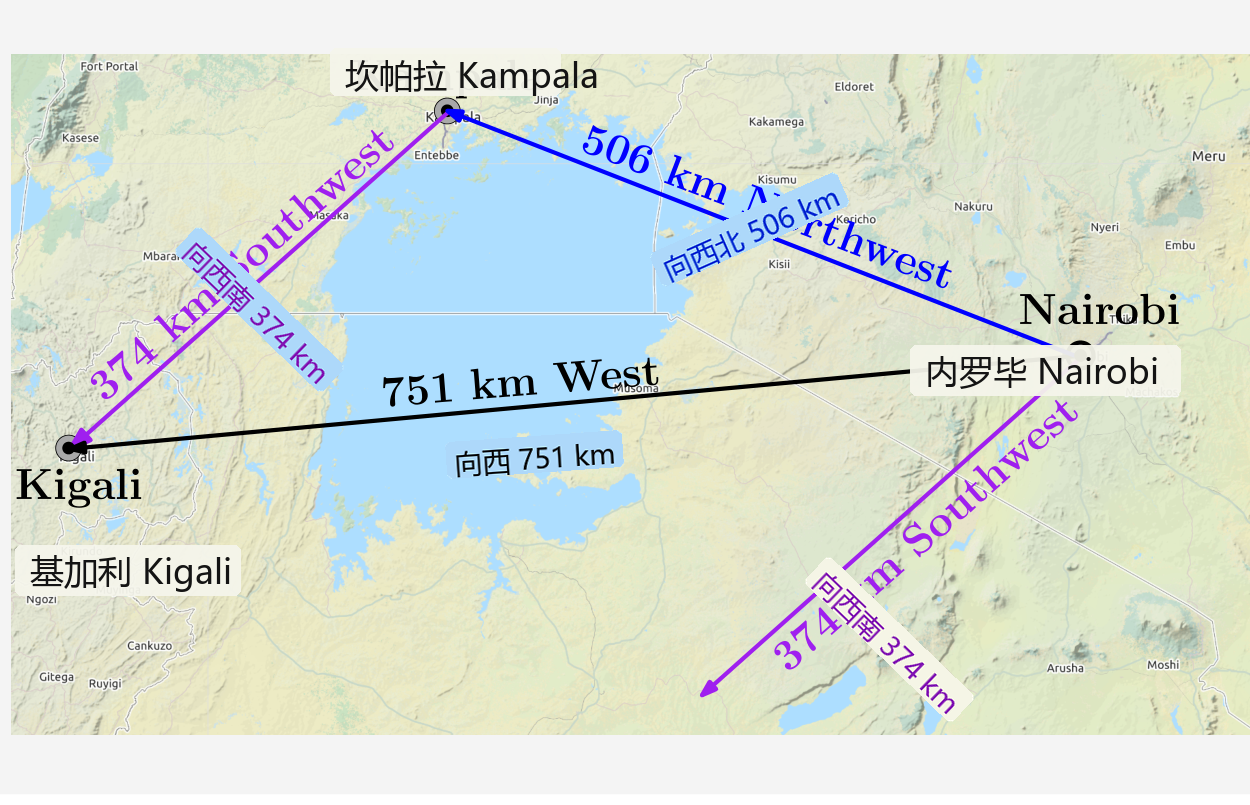
\includegraphics[width=0.92\textwidth,keepaspectratio]{docs/images/Figure2.7.png}
\caption*{\refstepcounter{figcounter}\label{fig:2-7}图~\thefigcounter 二维空间（平面）中线性相关向量的地理示例（粗略近似主要方位基向）。}
\end{figure}


\emph{备注} 。以下性质对于判断向量是否线性无关非常有用：

\begin{itemize}
\item $ k $ 个向量要么线性相关，要么线性无关，不存在第三种情况。
\item 如果向量 $ \boldsymbol{x}_1, \ldots, \boldsymbol{x}_k $ 中至少有一个是零向量 $ \boldsymbol{0} $，则它们线性相关。如果两个向量完全相同，结论同样成立。
\item 向量集合 $ \{\boldsymbol{x}_1, \ldots, \boldsymbol{x}_k : \boldsymbol{x}_i \neq \boldsymbol{0}, i = 1, \ldots, k\} $（$ k \geqslant 2 $）线性相关的充要条件是：其中（至少）有一个向量可以表示为其余向量的线性组合。特别地，如果一个向量是另一个向量的倍数（即 $ \boldsymbol{x}_i = \lambda \boldsymbol{x}_j, \lambda \in \mathbb{R} $），则该集合是线性相关的。
\end{itemize}

检验向量 $ \boldsymbol{x}_1, \ldots, \boldsymbol{x}_k \in V $ 是否线性无关的一种实用方法是使用高斯消元法：将所有向量作为矩阵 $ \boldsymbol{A} $ 的列，执行高斯消元直到该矩阵化为行阶梯形（此处不需要化为简化行阶梯形）：

\begin{itemize}
\item 主元列（pivot columns）表示与位于其左侧的向量线性无关的向量。请注意，在构建矩阵时向量之间存在先后顺序。
\item 非主元列可以表示为位于其左侧的主元列的线性组合。例如，行阶梯形： 告诉我们第一列和第三列是主元列。第二列是非主元列，因为它是第一列的 3 倍。
\end{itemize}
\begin{equation}
\begin{bmatrix} 1 & 3 & 0 \\ 0 & 0 & 2 \end{bmatrix}
\tag{2.66}\label{eq:2-66}
\end{equation}
\begin{itemize}
\item 所有列向量线性无关的充要条件是：所有列均为主元列。如果至少存在一个非主元列，则这些列（以及对应的向量）线性相关。
\end{itemize}

\begin{notebox}
\textbf{例 2.14}
\end{notebox}

\begin{notebox}
考虑 $ \mathbb{R}^4 $ 中的三个向量：

\begin{equation}
\boldsymbol{x}_1 = \begin{bmatrix} 1 \\ 2 \\ -3 \\ 4 \end{bmatrix}, \quad \boldsymbol{x}_2 = \begin{bmatrix} 1 \\ 1 \\ 0 \\ 2 \end{bmatrix}, \quad \boldsymbol{x}_3 = \begin{bmatrix} -1 \\ -2 \\ 1 \\ 1 \end{bmatrix}
\tag{2.67}\label{eq:2-67}
\end{equation}

为了检验它们是否线性相关，我们按照通用方法求解关于 $ \lambda_1, \lambda_2, \lambda_3 $ 的齐次方程：

\begin{equation}
\begin{adjustbox}{max width=\linewidth}
\lambda_1 \boldsymbol{x}_1 + \lambda_2 \boldsymbol{x}_2 + \lambda_3 \boldsymbol{x}_3 = \lambda_1 \begin{bmatrix} 1 \\ 2 \\ -3 \\ 4 \end{bmatrix} + \lambda_2 \begin{bmatrix} 1 \\ 1 \\ 0 \\ 2 \end{bmatrix} + \lambda_3 \begin{bmatrix} -1 \\ -2 \\ 1 \\ 1 \end{bmatrix} = \boldsymbol{0}
\end{adjustbox}
\tag{2.68}\label{eq:2-68}
\end{equation}

我们将向量 $ \boldsymbol{x}_i $（$ i = 1, 2, 3 $）按列拼成一个矩阵，并应用初等行变换，直到确定出主元列：

\begin{equation}
\begin{adjustbox}{max width=\linewidth}
\begin{bmatrix} 1 & 1 & -1 \\ 2 & 1 & -2 \\ -3 & 0 & 1 \\ 4 & 2 & 1 \end{bmatrix} \leadsto \cdots \leadsto \begin{bmatrix} 1 & 1 & -1 \\ 0 & 1 & 0 \\ 0 & 0 & 1 \\ 0 & 0 & 0 \end{bmatrix}
\end{adjustbox}
\tag{2.69}\label{eq:2-69}
\end{equation}

这里矩阵的每一列都是主元列。因此不存在非平凡解，解该方程组必须满足 $ \lambda_1 = 0, \lambda_2 = 0, \lambda_3 = 0 $。由此可知，向量 $ \boldsymbol{x}_1, \boldsymbol{x}_2, \boldsymbol{x}_3 $ 是线性无关的。
\end{notebox}

\emph{备注} 。考虑一个具有 $ k $ 个线性无关向量 $ \boldsymbol{b}_1, \ldots, \boldsymbol{b}_k $ 的向量空间 $ V $，以及 $ m $ 个线性组合：

\begin{equation}
\begin{aligned}
  \boldsymbol{x}_1 &= \sum_{i=1}^k \lambda_{i1} \boldsymbol{b}_i \\
  &\ \ \vdots \\
  \boldsymbol{x}_m &= \sum_{i=1}^k \lambda_{im} \boldsymbol{b}_i
\end{aligned}
\tag{2.70}\label{eq:2-70}
\end{equation}

将以这些线性无关向量 $ \boldsymbol{b}_1, \ldots, \boldsymbol{b}_k $ 为列的矩阵定义为 $ \boldsymbol{B} = [\boldsymbol{b}_1, \ldots, \boldsymbol{b}_k] $，我们可以将上述线性组合更紧凑地写为：

\begin{equation}
\boldsymbol{x}_j = \boldsymbol{B} \boldsymbol{\lambda}_j, \quad \boldsymbol{\lambda}_j = \begin{bmatrix} \lambda_{1j} \\ \vdots \\ \lambda_{kj} \end{bmatrix}, \quad j = 1, \ldots, m
\tag{2.71}\label{eq:2-71}
\end{equation}

我们想要检验 $ \boldsymbol{x}_1, \ldots, \boldsymbol{x}_m $ 是否线性无关。为此，我们按照通用方法检验何时 $ \sum_{j=1}^m \psi_j \boldsymbol{x}_j = \boldsymbol{0} $。结合 (2.71)，我们得到：

\begin{equation}
\sum_{j=1}^m \psi_j \boldsymbol{x}_j = \sum_{j=1}^m \psi_j \boldsymbol{B} \boldsymbol{\lambda}_j = \boldsymbol{B} \sum_{j=1}^m \psi_j \boldsymbol{\lambda}_j
\tag{2.72}\label{eq:2-72}
\end{equation}

这意味着，向量集合 $ \{\boldsymbol{x}_1, \ldots, \boldsymbol{x}_m\} $ 线性无关的充要条件是：列向量集合 $ \{\boldsymbol{\lambda}_1, \ldots, \boldsymbol{\lambda}_m\} $ 线性无关。

\emph{备注} 。在向量空间 $ V $ 中，$ k $ 个向量 $ \boldsymbol{x}_1, \ldots, \boldsymbol{x}_k $ 的 $ m $ 个线性组合在 $ m > k $ 时必定线性相关。

\begin{notebox}
\textbf{例 2.15}
\end{notebox}

\begin{notebox}
考虑一组线性无关的向量 $ \boldsymbol{b}_1, \boldsymbol{b}_2, \boldsymbol{b}_3, \boldsymbol{b}_4 \in \mathbb{R}^n $，以及：

\begin{equation}
\begin{adjustbox}{max width=\linewidth}
\begin{aligned}
  \boldsymbol{x}_1 &= \boldsymbol{b}_1 - 2\boldsymbol{b}_2 + \boldsymbol{b}_3 - \boldsymbol{b}_4 \\
  \boldsymbol{x}_2 &= -4\boldsymbol{b}_1 - 2\boldsymbol{b}_2 + 4\boldsymbol{b}_4 \\
  \boldsymbol{x}_3 &= 2\boldsymbol{b}_1 + 3\boldsymbol{b}_2 - \boldsymbol{b}_3 - 3\boldsymbol{b}_4 \\
  \boldsymbol{x}_4 &= 17\boldsymbol{b}_1 - 10\boldsymbol{b}_2 + 11\boldsymbol{b}_3 + \boldsymbol{b}_4
\end{aligned}
\end{adjustbox}
\tag{2.73}\label{eq:2-73}
\end{equation}

向量 $ \boldsymbol{x}_1, \ldots, \boldsymbol{x}_4 \in \mathbb{R}^n $ 是否线性无关？
\end{notebox}

\begin{notebox}
为了回答这个问题，我们研究列向量集合：

\begin{equation}
\left\{ \begin{bmatrix} 1 \\ -2 \\ 1 \\ -1 \end{bmatrix}, \begin{bmatrix} -4 \\ -2 \\ 0 \\ 4 \end{bmatrix}, \begin{bmatrix} 2 \\ 3 \\ -1 \\ -3 \end{bmatrix}, \begin{bmatrix} 17 \\ -10 \\ 11 \\ 1 \end{bmatrix} \right\}
\tag{2.74}\label{eq:2-74}
\end{equation}

是否线性无关。对应线性方程组的系数矩阵为：

\begin{equation}
\begin{adjustbox}{max width=\linewidth}
\boldsymbol{A} = \begin{bmatrix} 1 & -4 & 2 & 17 \\ -2 & -2 & 3 & -10 \\ 1 & 0 & -1 & 11 \\ -1 & 4 & -3 & 1 \end{bmatrix}
\end{adjustbox}
\tag{2.75}\label{eq:2-75}
\end{equation}

将其化为简化行阶梯形矩阵，结果为：

\begin{equation}
\begin{adjustbox}{max width=\linewidth}
\begin{bmatrix} 1 & 0 & 0 & -7 \\ 0 & 1 & 0 & -15 \\ 0 & 0 & 1 & -18 \\ 0 & 0 & 0 & 0 \end{bmatrix}
\end{adjustbox}
\tag{2.76}\label{eq:2-76}
\end{equation}

我们看到对应的线性方程组具有非平凡解：最后一列不是主元列，并且 $ \boldsymbol{x}_4 = -7\boldsymbol{x}_1 - 15\boldsymbol{x}_2 - 18\boldsymbol{x}_3 $。因此，$ \boldsymbol{x}_1, \ldots, \boldsymbol{x}_4 $ 是线性相关的，因为 $ \boldsymbol{x}_4 $ 可以表示为 $ \boldsymbol{x}_1, \ldots, \boldsymbol{x}_3 $ 的线性组合。
\end{notebox}
